\documentclass{beamer}
\usepackage[utf8]{inputenc}
%\usepackage[ngerman]{babel}

\usepackage{graphicx}
\usepackage{booktabs}
\usetheme{tud}
\usefonttheme{tud}

\usepackage[T1]{fontenc}
\usepackage{amsmath}
\usepackage{mathtools}
\usepackage{amssymb}
\usepackage{amsfonts}
\usepackage{amsthm}
\usepackage{mathabx}
\usepackage[utf8]{inputenc}
\usepackage[T1]{fontenc}
\usepackage[style=numeric]{biblatex}
\usepackage{algorithm}   % for typesetting algorithms
\usepackage{algorithmic} % for typesetting algorithms in pseudocode


\addbibresource{refs.bib}



\DeclareMathOperator{\st}{st}

\newcommand*{\textcal}[1]{%
  % family qzc: Font TeX Gyre Chorus (package tgchorus)
  % family pzc: Font Zapf Chancery (package chancery)
  \textit{\fontfamily{qzc}\selectfont#1}%
}

\usepackage{tikz}
\usepackage{forest}
\usetikzlibrary{shapes.geometric, arrows}


%TIKZ STYLES
\tikzstyle{flownode} = [rectangle, rounded corners, minimum width=2cm,
minimum height=1cm, text centered, draw=black, scale=0.85]

\tikzstyle{arrow} = [thick,->,>=stealth]

\tikzstyle{node} = [circle, draw=black]
\tikzstyle{edge} = [thick,-,>=stealth]
\tikzstyle{box} = [rectangle,text centered,draw=black, minimum width = 2cm,
minimum height=1cm]
\tikzstyle{dia} = [diamond, text centered, draw=black,
minimum width=2cm, minimum height=1cm]
%\usepackage{tikz-uml}
%\usepackage{scalefnt}
%\usepackage{hyperref}
%\usepackage{pgfplots}
%\usepackage{csquotes}

\title{Generating Proofs in the Description Logic ALCH}
\author{Steffen Breuer}
\institute[Automata Theory]{TU Dresden}

\begin{document}
\maketitle

%\begin{frame}
%\frametitle{Content}
%\tableofcontents
%\end{frame}

\section{Introduction}
\begin{frame}
\frametitle{Motivation}
    \begin{itemize}
        \item Debugging of ontologies
        \item Understanding results
    \end{itemize}
\end{frame}

\begin{frame}
\frametitle{Description Logic $\mathcal{ALCH}$}    
\begin{itemize}
        \item negation ($\neg$)
        \item concept intersection ($\sqcap$)
        \item concept union ($\sqcup$)
        \item value restriction ($\forall$)
        \item existential restriction ($\exists$)
        \item top concept ($\top$)
        \item bottom concept ($\bot$)
        \item gerneral concept inclusion ($C \sqsubseteq D$)
        \item role inclusion ($ r \sqsubseteq s$)
    \end{itemize}
\end{frame}

\begin{frame}
\frametitle{Semantics}
Let $A \in N_C, C, D \in N_{\mathcal{ALCH}}, r \in N_R$ then
  \begin{center}
    \begin{tabular}{l c l}
      %use align* * := ohne nummerierung
    
      $\top^I$& $\coloneqq$& $\Delta^I$ \\
      $\bot^I$& $\coloneqq$& $\emptyset$\\      
      %$A^I$ & $\coloneqq$ & $A'$ where $A' \subseteq \Delta^I$ \\
      %$r^I$ & $\coloneqq$ & $R$ where $R \subseteq \Delta^I \times \Delta^I$\\
      $(\neg C)^I$ & $\coloneqq$ & $C^I$ \\
      $(C \sqcap D)^I$ & $\coloneqq$ & $C^I \cap D^I$ \\
      $(C \sqcup D)^I$ & $\coloneqq$ & $C^I \cup D^I$ \\
      $(\exists r.C)^I$ & $\coloneqq$ & $ \{a \in \Delta^I \mid \exists b \in \Delta^I : (a,b) \in r^I \text{ and } b \in C^I \}$ \\
      $(\forall r.C)^I$ & $\coloneqq$ & $ \{a \in \Delta^I \mid \forall b \in \Delta^I : \text{if} (a,b) \in r^I \text{, then } b \in C^I \}$ \\
      \end{tabular}        
  \end{center}
\end{frame}

\begin{frame}
    \frametitle{Semantics}
    \begin{itemize}
        \item For $C, D \in N_{\mathcal{ALCH}}: I \models C \sqsubseteq D  :\iff C^I \subseteq D^I$ \\
        \item For $r, s \in N_R: I \models r \sqsubseteq s  :\iff r^I \subseteq s^I$
    \end{itemize}
    
   
\end{frame}

\begin{frame}
\frametitle{Proofs}
\begin{itemize}
    \item $G = (V, E, l)$ finite, acyclic, directed, labeled hypergraph
    \begin{itemize}
        \item $V$ set of nodes
        \item $E \subseteq V^n$ set of hyperedges 
        \item $l: V \rightarrow \mathcal{L}$ labeling function such that $\{l(v) \mid v \in S \} \models l(d)$
    \end{itemize}
\end{itemize}
\end{frame}

\begin{frame}
    \frametitle{}
    \begin{figure}
        
        \centering
        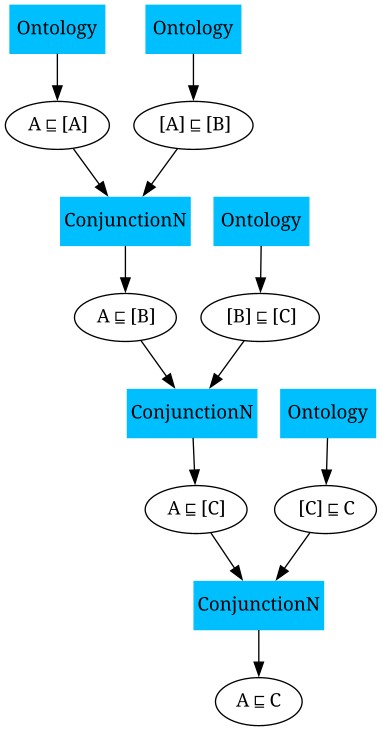
\includegraphics[width=0.30\textwidth]{pictures/longerProofExample2_normalized.png}
        \caption{$\mathcal{O} \coloneq \{A \sqsubseteq B , B \sqsubseteq C \}$, Goal: $A \sqsubseteq C$}
    
    \end{figure}
     
 \end{frame}

\begin{frame}
\frametitle{The Algorithm}
\begin{itemize}
    \item Normalization
    \item Rule Application
    \item Proof Extraction
\end{itemize}
\end{frame}

\begin{frame}
\frametitle{Normal Form}
\begin{itemize}
    \item $ \bigsqcap A_i \sqsubseteq \bigsqcup B_j$
    \item $A \sqsubseteq \exists r.B$
    \item $\exists r.A \sqsubseteq A$
    \item $A \sqsubseteq \forall r.B$
    \item $r \sqsubseteq s$
\end{itemize}
  
\end{frame}

\begin{frame}
\frametitle{Normalization}
\begin{enumerate}
    \item removal of axioms with negative $\forall r.C$ as subconcept
    \item apply structural transformation
    \item final normalization rules
\end{enumerate}
\end{frame}

\begin{frame}
    \frametitle{Positive and Negative Occurrences Of Concepts}
  Let $\mathcal{O} = (\mathcal{T}, \mathcal{A})$ some ontology and $C$ some concept then we say that a concept $C$ occurs positively (negatively) in $\mathcal{O}$ if
  $C$ occurs positively (negatively) in some GCI of $\mathcal{T}$. \\
  \begin{itemize}
    \item $C$ occurs positively in itself.
    \item If $C$ occurs positively (negatively) in C' then C occurs positively (negatively) in
    $C' \sqcap D C \sqcap D', C' \sqcup D, C \sqcup D', \exists r.C', \forall r.C', D \sqsubseteq C'$ 
    and negatively (positively) in $\neg C',C' \sqsubseteq D$.
  \end{itemize}
    
  
    \end{frame}

\begin{frame}
\frametitle{Structural Transformation}
\begin{center}

    \begin{tabular}{l l }
    $\st(A) \coloneqq  A$ & $\st(C \sqcap D) \coloneqq  [C] \sqcap [D]$\\
    $\st(\top) \coloneqq \top$ & $\st(C \sqcup D) \coloneqq [C] \sqcup [D]$ \\
    $\st(\bot) \coloneqq \top$ & $\st(\exists r.C) \coloneqq \exists r.[C]$\\
    $\st(\neg C) \coloneqq \neg [C]$ & $\st(\exists r.C) \coloneqq \exists r.[C]$\\
    \end{tabular}
    
    \end{center}
\end{frame}

\begin{frame}
    \frametitle{Structural Transformation}
        \begin{itemize}
            \item $ \st(C) \sqsubseteq [C]$ for every negative $C$ in $\mathcal{O}$ 
            \item $ [D]\sqsubseteq \st(D)$ for every positive $D$ in $\mathcal{O}$
            \item $ [C] \sqsubseteq [D]$ for every axiom $C \sqsubseteq D$ occurring in$ \mathcal{O}$
          \end{itemize}
    \end{frame}



\begin{frame}
\frametitle{Normalization Rules}
\begin{center}
    \begin{itemize}
        \item $ \dfrac{[C \sqcap D] \sqsubseteq [C] \sqcap [D]}{ [C \sqcap D] \sqsubseteq [C], \quad [C \sqcap D] \sqsubseteq [D]}$
        \item $ \dfrac{[C] \sqcup [D] \sqsubseteq [C \sqcup D]}{ [C] \sqsubseteq [C \sqcup D], \quad [D] \sqsubseteq [C \sqcup D]}$
        \item $ \dfrac{[\neg C] \sqsubseteq \neg [C] }{ [\neg C ] \sqcap [C] \sqsubseteq \bot}$
        \item $ \dfrac{\neg [C] \sqsubseteq [\neg C] }{ \top \sqsubseteq [\neg C ] \sqcap [C]}$
      \end{itemize}
\end{center}
\end{frame}

\begin{frame}
\frametitle{Rule Application}


  
  \textbf{Procedure} \textsc{main}$(\text{ontology}, \text{goal})$\\
  \hspace*{1em} \textbf{1.} \textsc{Normalizer.normalize}$(\text{ontology})$\\
  \hspace*{1em} \textbf{2.} $\text{proofHandler} \gets \text{new ProofHandler}(\text{goal})$\\
  \hspace*{1em} \textbf{3.} $\text{rules} \gets \text{getRules}(\text{ontology}, \text{proofHandler})$\\
  \hspace*{1em} \textbf{4.} \textbf{while} notFinished$(\text{proofHandler})$ \textbf{do}\\
  \hspace*{2em} \textbf{5.} \textbf{for} $(\text{rule in rules})$ \textbf{do}\\
  \hspace*{3em} \textbf{6.} $\text{setNewRule}(\text{rule.apply}())$\\
  


\end{frame}

\begin{frame}
    \frametitle{Proof Handler}
    \begin{itemize}
        \item Active Axioms
        \item Active Concepts
        \item Inference Handling
        \item Goal Checking
        \item Proof Extraction
    \end{itemize}
      
    
    \end{frame}

\begin{frame}
\frametitle{Rules}
{\small
\begin{align}
    \mathbf{R^{+}_A} & \dfrac{}{H\sqsubseteq A} : A \in H \label{rules:RPlusA}\\
    \mathbf{R^{-}_A} & \dfrac{H \sqsubseteq N \sqcup A}{H \sqsubseteq N} : \neg A \in H  \label{rules:RMinusA}\\ 
    \mathbf{R^{n}_{\sqcap}} & \dfrac{\{H \sqsubseteq N_i \sqcup A_i \}^{n}_{i=1}}{H \sqsubseteq \bigsqcup^{n}_{i=1} N_i \sqcup M} : \bigsqcap^{n}_{i=1} A_i \sqsubseteq M \in \mathcal{O} \label{rules:RNAnd} \\
    \mathbf{R^+_{\exists}} & \dfrac{H \sqsubseteq N \sqcup A }{ H \sqsubseteq N \sqcup \exists r.B} : A \sqsubseteq \exists r.B \in \mathcal{O} \label{rules:RPlusExists}\\
    \mathbf{R^-_{\exists}} & \dfrac{H \sqsubseteq M \sqcup \exists r.K,\quad K \sqsubseteq N \sqcup A}{H \sqsubseteq M \sqcup B \sqcup \exists r.(K \sqcap \neg A)} : \exists s.A \sqsubseteq B \in \mathcal{O} \quad r \sqsubseteq_{\mathcal{O}} s \label{rules:RMinusExists}\\
    \mathbf{R^\bot_{\exists}} & \dfrac{H \sqsubseteq M \sqcup \exists r.K,\quad K \sqsubseteq \bot}{H \sqsubseteq M} \label{rules:RBotExists}\\
    \mathbf{R_{\forall}} & \dfrac{H \sqsubseteq M \sqcup \exists r.K,\quad H \sqsubseteq N \sqcup A}{H \sqsubseteq M \sqcup N \sqcup \exists r.(K \sqcap B)} : A \sqsubseteq \forall s.B \in \mathcal{O} \quad r \sqsubseteq_{\mathcal{O}} s \label{rules:RForall}
  \end{align}
}
{\tiny Consequence-Based Reasoning beyond Horn Ontologies \cite{10.5555/2283516.2283580}}

\end{frame}

\begin{frame}
\frametitle{$\mathbf{R^{+}_A} \coloneq \dfrac{}{H\sqsubseteq A} : A \in H$}
\begin{itemize}
    \item ontology independent
    \item uses active concepts
    \item active concepts can be removed
\end{itemize}
\end{frame}

\begin{frame}
    \frametitle{$\mathbf{R^{-}_A} \coloneq \dfrac{H \sqsubseteq N \sqcup A}{H \sqsubseteq N} : \neg A \in H$}
    \begin{itemize}
        \item ontology independent
        \item uses active axioms
        \item Search
        \begin{enumerate}
            \item search for axiom with $\neg A \in H$ (find all)
            \item check whether $A$ in superconcept 
        \end{enumerate}
    \end{itemize}
\end{frame}

\begin{frame}
    \frametitle{$\mathbf{R^{n}_{\sqcap}} \coloneq \dfrac{\{H \sqsubseteq N_i \sqcup A_i \}^{n}_{i=1}}{H \sqsubseteq \bigsqcup^{n}_{i=1} N_i \sqcup M} : \bigsqcap^{n}_{i=1} A_i \sqsubseteq M \in \mathcal{O}$}
    \begin{itemize}
        \item filter ontology
        \begin{itemize}
            \item list of tuples $(\{A_1,\ldots A_n\}, \bigsqcap^{n}_{i=1} A_i \sqsubseteq M)$
        \end{itemize}
        \item preprocess active axioms
        \begin{itemize}
            \item $m(H,A) \coloneqq \langle (\{N_c \mid N_c \in N\}, H \sqsubseteq N \sqcup A)\rangle$
        \end{itemize} 
        \item search
        \begin{enumerate}
            \item check for each H if $\{A \mid m(H,A) \text{ defined} \} \subseteq \{A_1, \ldots, A_n\}$
            \item create all $n^{\sum_{i=1}^{n}|m(H,A_i)|}$ combinations of $H \sqsubseteq \bigsqcup^{n}_{i=1} N_i \sqcup M$
            
        \end{enumerate}
    \end{itemize}

\end{frame}

\begin{frame}
    \frametitle{$\mathbf{R^+_{\exists}} \coloneq \dfrac{H \sqsubseteq N \sqcup A }{ H \sqsubseteq N \sqcup \exists r.B} : A \sqsubseteq \exists r.B \in \mathcal{O}$}
    \begin{itemize}
        \item filter ontology for $A \sqsubseteq \exists r.B$
        \item for each $A$ in ontology search for $H \sqsubseteq N \sqcup A$
    \end{itemize}
\end{frame}

    \begin{frame}
        %\frametitle{$\mathbf{R^-_{\exists}} \coloneq \dfrac{H \sqsubseteq M \sqcup \exists r.K,\quad K \sqsubseteq N \sqcup A}{H \sqsubseteq M \sqcup B \sqcup \exists r.(K \sqcap \neg A)} : \newline  \exists s.A \sqsubseteq B \in \mathcal{O} \quad r \sqsubseteq_{\mathcal{O}} s$}
        \frametitle{
            \begin{tabular}{ll}
                $\mathbf{R^-_{\exists}} \coloneq $&$\dfrac{H \sqsubseteq M \sqcup \exists r.K,\quad K \sqsubseteq N \sqcup A}{H \sqsubseteq M \sqcup B \sqcup \exists r.(K \sqcap \neg A)} :$\\
                &$A \sqsubseteq \forall s.B \in \mathcal{O} \quad r \sqsubseteq_{\mathcal{O}} s$
            \end{tabular}
          }
        
        \begin{itemize}
            \item filter ontology for $r$ and $A$ combinations
            \item search $K \sqsubseteq N \sqcup A$ for some $A$
            \item for found K search for $H \sqsubseteq M \sqcup \exists r.K$
        \end{itemize}
    \end{frame}
    
        \begin{frame}
            \frametitle{$\mathbf{R^\bot_{\exists}} \coloneq \dfrac{H \sqsubseteq M \sqcup \exists r.K,\quad K \sqsubseteq \bot}{H \sqsubseteq M}$}
            \begin{itemize}
                \item ontology independent
                \item first search for $K$ then for $H$
            \end{itemize}
        \end{frame}

            \begin{frame}
                %\frametitle{$\mathbf{R_{\forall}} \coloneq \dfrac{H \sqsubseteq M \sqcup \exists r.K,\quad H \sqsubseteq N \sqcup A}{H \sqsubseteq M \sqcup N \sqcup \exists r.(K \sqcap B)} : \newline A \sqsubseteq \forall s.B \in \mathcal{O} \quad r \sqsubseteq_{\mathcal{O}} s$}
                \frametitle{
    \begin{tabular}{ll}
      $\mathbf{R_{\forall}} \coloneq$ & $\dfrac{H \sqsubseteq M \sqcup \exists r.K,\quad H \sqsubseteq N \sqcup A}{H \sqsubseteq M \sqcup N \sqcup \exists r.(K \sqcap B)}:$ \\
      &$A \sqsubseteq \forall s.B \in \mathcal{O} \quad r \sqsubseteq_{\mathcal{O}} s$
    \end{tabular}
  }
                \begin{itemize}
                    \item filter ontology for $r$ and $A$ combinations
                    \item for each $(A, r)$ search for $H \sqsubseteq N \sqcup A$
                    \item based on $H$ search for $H \sqsubseteq M \sqcup \exists r.K$
                \end{itemize}    
            \end{frame}

            \begin{frame}
                \frametitle{Comparison to Lethe }
                 \begin{itemize}
                        \item LetheBasedALCHProofGenerator
                        \item elimination based
                        \item different calculus \cite{KoopmannSchmidt15c}
                        \item also uses EVEE \cite{https://doi.org/10.48550/arxiv.2206.07711}
                        \begin{itemize}
                            \item https://github.com/de-tu-dresden-inf-lat/evee
                        \end{itemize}
                        \item tasks \cite{10.1007/978-3-031-10769-6_16}
                 \end{itemize}
             \end{frame}

             \begin{frame}
                \frametitle{Task 1}
                    \begin{itemize}
                    \item $\mathcal{O} \coloneq \{A \sqsubseteq C , C \sqsubseteq D, D \sqsubseteq E, B \equiv (F \sqcap \exists s. \exists r.G), A \sqsubseteq \exists s. \exists r.G, \newline E \equiv ((D \sqcup H \sqcup I) \sqcap F)\}$ \\
                    \item Goal: $A \sqsubseteq B$
                    \end{itemize}
                    

            \end{frame}
                

            \begin{frame}
                \frametitle{}               
                \begin{figure}
                    \centering
                    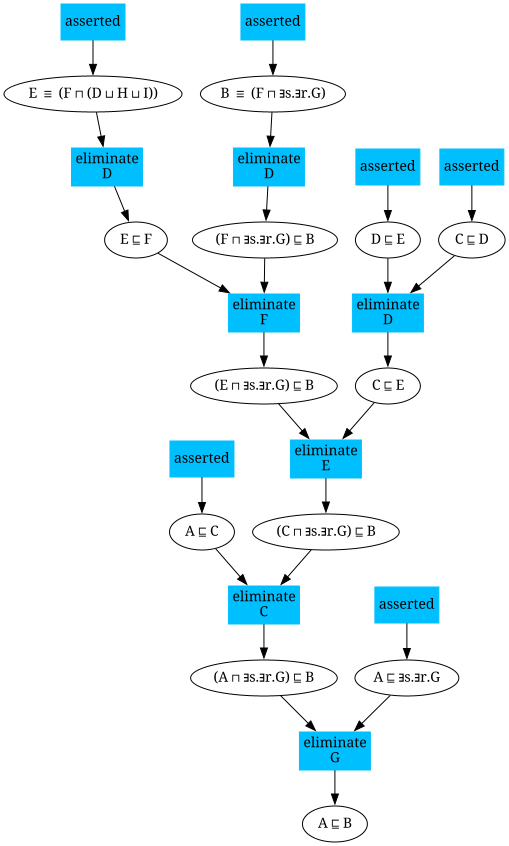
\includegraphics[width=0.37\textwidth]{pictures/Lethe_task00001.png}
                    \caption{Lethe Proof for Task 1}
                  \end{figure}
             \end{frame}
            \begin{frame}
                \frametitle{}
                \begin{figure}
                    \centering
                    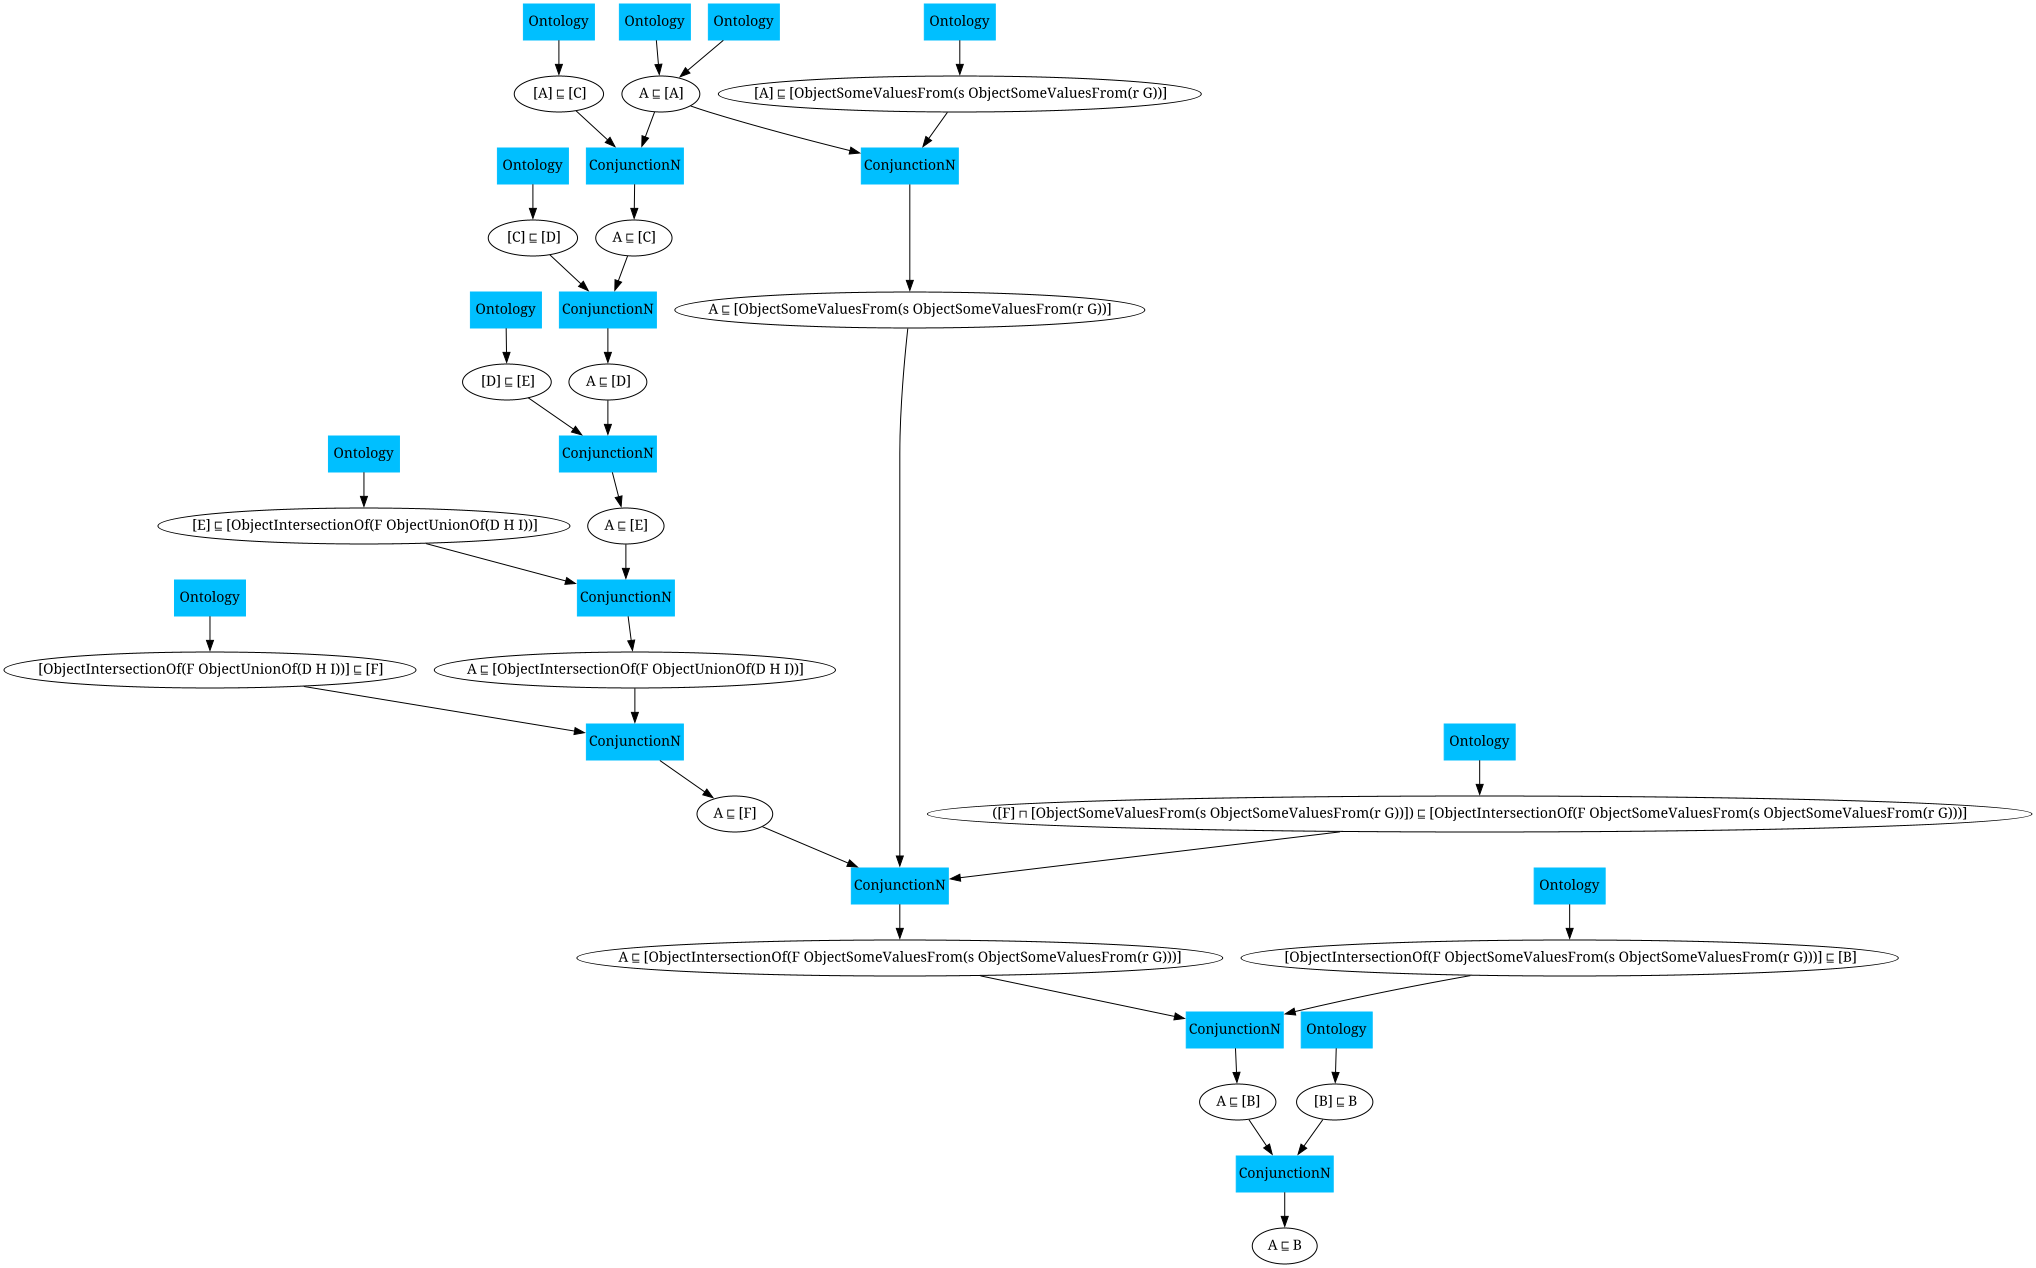
\includegraphics[width=1\textwidth]{pictures/ALCH_task00001.png}
                    \caption{ALCH-Reasoner Proof for Task 1}
                  \end{figure}
             \end{frame}

             %%%
             \begin{frame}
                \frametitle{Task 3}
                    \begin{itemize}
                    \item $\mathcal{O} \coloneq \{A \equiv (C \sqcap \exists r.(D \sqcap \forall s.E)) , B \equiv (\exists r.D \sqcap C) \}$ \\
                    \item Goal: $A \sqsubseteq B$
                    \end{itemize}
                    

            \end{frame}
                

            \begin{frame}
                \frametitle{}               
                \begin{figure}
                    \centering
                    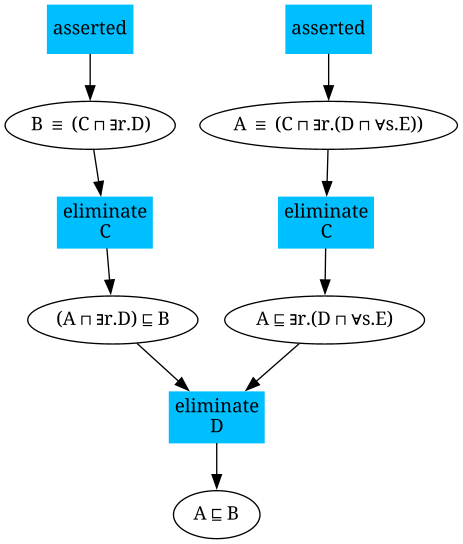
\includegraphics[width=0.37\textwidth]{pictures/Lehte_task00003.png}
                    \caption{Lethe Proof for Task 3}
                  \end{figure}
             \end{frame}
             
            \begin{frame}
                \frametitle{}
                \begin{figure}
                    \centering
                    
\includegraphics[width=1\textwidth]{pictures/ALCH_task00003.png}
                    \caption{ALCH-Reasoner Proof for Task 3}
                  \end{figure}
             \end{frame}

            %%%
            \begin{frame}
                \frametitle{}
                \begin{figure}
                    
                    \centering
                    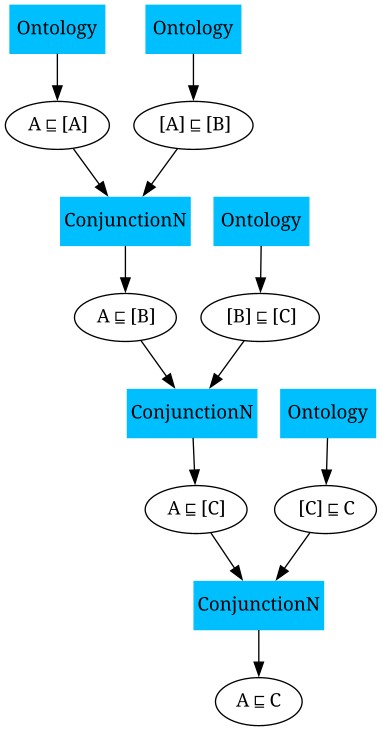
\includegraphics[width=0.30\textwidth]{pictures/longerProofExample2_normalized.png}
                    \caption{$\mathcal{O} \coloneq \{A \sqsubseteq B , B \sqsubseteq C \}$, Goal: $A \sqsubseteq C$}
                
                \end{figure}
                 
             \end{frame}
             
             \begin{frame}
                \frametitle{ALCH-Reasoner Performance}

                {\footnotesize
                
                \begin{table}[h]
                    \centering
                    \begin{tabular}{|c|c|c|c|c|}
                      \hline
                      \textbf{Task} & \textbf{Time (ms)} & \textbf{\#Axioms} & \textbf{Size largest Premise} & \textbf{\#RuleApplications} \\
                      \hline
                      00001 & 192 & 19 & 3 & 20  \\
                      00003 & 5913 & 23 & 4 & 27 \\
                      00008 & 133 & 15 & 3 & 18  \\
                      00009 & 119 & 25 & 4 & 27  \\
                      00012 & 24 & 7 & 2 & 7  \\
                      \hline
                    \end{tabular}
                  \end{table}
                  }
             \end{frame}

             \begin{frame}
                \frametitle{Lethe Performance}

                {\footnotesize
                
                \begin{table}[h]
                    \centering
                    \begin{tabular}{|c|c|c|c|c|}
                      \hline
                      \textbf{Task} & \textbf{Time (ms)} & \textbf{\#Axioms} & \textbf{Size largest Premise} & \textbf{\#RuleApplications} \\
                      \hline
                      \hline
                      00001 & 2786 & 13 & 2 & 13 \\
                      00003 & 502 & 5 & 2 & 5  \\
                      00008 & 2728 & 8 & 2 & 8  \\
                      00009 & 1348 & 11 & 2 & 11 \\
                      00012 & 159 & 2 & 1 & 2  \\
                      \hline
                    \end{tabular}
                  \end{table}
                  }
             \end{frame}

             \begin{frame}
                \frametitle{Conclusion}
                \begin{itemize}
                    \item Removal of normalization-caused steps
                    \item Less readable due to normalization
                    \item Fast but can be optimized
                \end{itemize}
                 
             \end{frame}

             \begin{frame}
                \begin{center}
                    \Huge Thank you for your attention!
                \end{center}
                 
             \end{frame}
             
                
\end{document}